\scanpage{8}
\mspage{0}
XII\quad \uline{Tores maximaux}, \uline{groupe de Weyl}, \uline{sous-groupes de Cartan}, \uline{centre
réductif des schémas en groupes lisses et affines}.

par A. Grothendieck.

A partir du présent exposé, contrairement aux exposés précédents,
nous ferons usage des résultats connus sur la structure des groupes
algébriques lisses sur un corps algébriquement clos k, et surtout
de la théorie de BOREL des groupes algébriques affines, exposée dans
le Séminaire CHEVALLEY 56/57: \deleted{sur les Groupes} ``Classification des
groupes de Lie Algébriques''. Suivant l'usage en théorie des groupes
algébriques, nous référons à ce Séminaire par le sigle BIBLE. Pour les
\deleted{moment,}\inserted{prochains exposés,} nous aurons besoin \inserted{notamment} des résultats de\deleted{s} BIBLE 4, 5, 6, 7
(le chiffre après BIBLE renvoie au numéro de l'exposé). Il \deleted{\unsure{me}} semble
\deleted{\illegible{1}}\inserted{d'ailleurs} que la théorie des schémas \inserted{n'}apporte aucune simplification notable
à la théorie \deleted{exposée} de BOREL \deleted{\unsure{en question}} telle qu'elle est exposée
dans BIBLE. C'est pourquoi il n'a pas semblé utile de la reproduire \deleted{ici}
\deleted{notre objet étant} dans le présent Séminaire, notre but étant ici de
déduire, de résultats connus sur les corps algébriquement clos, des
résultats analogues valables sur tout préschéma de base. (Il n'en sera
plus de même pour la théorie de structure de CHEVALLEY des groupes
semi-simples, qui, semble-t-il, se traite avec avantage ab ovo sur un
préschéma de base quelconque).

\inserted{Dans les exposés oraux \inserted{(que nous avons suivi dans les N°s 1 à 4)}
nous nous étions limités aux
préschémas en groupes affines sur S, en nous appuyant
de façon essentielle sur les théorèmes de représentabilité
de Exp \uline{XI} N°4. Dans les présentes notes (cf
N°s 6 à \unsure{8}) nous montrons rapidement comment on peut
éliminer les hypothèses affines \deleted{\unsure{par une méthode plus}}
\inserted{par une \deleted{\illegible{1}} méthode} plus
simple n'utilisant pas les résultats les plus délicats de Exp. \uline{XI}.}
\figure{
\begin{tikzpicture}[baseline]\draw (0,0) circle (.055);\draw (0,.055)--(.18,.5);\end{tikzpicture}}

\margin{Pour d'autres généralisations des résultats contenus
dans le présent exposé, voir également exposés
\deleted{\unsure{Exp.}}\uline{XV} et \uline{XVI}. (Il est évident que le contenu des
exposés \uline{XI}, \uline{XII}, \uline{XV}, \uline{XVI} devrait être complètement refondu).}
\margin{\figure{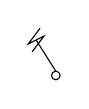
\begin{tikzpicture}[baseline]\draw (0,0) circle (.055);\draw (0,.055)--(-.25,.45);\draw (-.3,.3)--(-.15,.5)--(-.35,.4)--(-.2,.6);\end{tikzpicture}}}
\margin{7}
